\chapter{Procedures and the Stack}

\section*{Learning Objectives}
After completing this experiment, you will be able to:
\begin{itemize}[nosep]
  \item Call and return from procedures using \texttt{BL} and \texttt{BX LR}.
  \item Apply the ARM Procedure Call Standard (AAPCS) to pass parameters, return results, and decide which registers must be preserved.
  \item Use \texttt{PUSH} and \texttt{POP} to save and restore callee-saved registers and \texttt{LR} on the full descending stack.
  \item Implement nested and recursive procedures that manage the stack correctly.
\end{itemize}

\section*{Experiment Overview}
This experiment builds on the branching and loop patterns from Experiment 3 to write modular assembly code. You will define procedures, follow the AAPCS calling convention for arguments, return values, and register preservation, and use the stack to save the return address and working registers across nested and recursive calls. By the end of this lab, you will be able to split a program into reusable procedures that call each other safely.

\newpage

\section{Theoretical Background}
\subsection{ARM Architecture Procedure Call Standard (AAPCS)}

Procedures are reusable blocks of code that encapsulate a specific task. They promote modular design, code reuse, and clearer program structure. In ARM assembly, procedures are implemented using branch-and-link instructions along with register usage conventions defined by the ARM Architecture Procedure Call Standard (AAPCS).

The AAPCS is the set of rules that define how functions exchange data and how registers must be preserved during a procedure call:

\begin{itemize}[nosep]
  \item \textbf{R0--R3}: Hold the first four parameters. \texttt{R0} also holds the return value. Caller-saved.
  \item \textbf{Stack}: Any additional parameters beyond the first four are passed on the stack.
  \item \textbf{R4--R11}: Must be preserved by the callee. If a procedure uses them, it must save and restore them.
  \item \textbf{R12 (IP)}: Intra-procedure-call scratch register. Caller-saved — a callee may freely overwrite it, so (like R0--R3) never assume it survives a \texttt{BL}.
  \item \textbf{SP (R13)}: Stack pointer, always points to the current top of the stack.
  \item \textbf{LR (R14)}: Link register holds the return address. Caller-saved.
\end{itemize}
\paragraph{Note:} Callees are the procedures being called, while callers are the ones calling the procedure.

\subsection{Procedure Templates}

A procedure is entered with a \texttt{BL} (branch-with-link) instruction, which stores the return address in the link register \texttt{LR}. The callee returns by branching to \texttt{LR} (e.g., \texttt{BX LR}). By the AAPCS, the first four arguments are passed in \texttt{R0--R3} and the primary return value is placed in \texttt{R0}.
\newpage
\paragraph{Basic Procedure Template}

\paragraph{Example:} simple procedure that expects two integers in \texttt{R0} and \texttt{R1} and returns their sum in \texttt{R0}.

\begin{lstlisting}[caption={Basic procedure structure}]
AddTwo  PROC
        ADD R0, R0, R1   ; return R0+R1 in R0
        BX  LR
        ENDP
\end{lstlisting}
\paragraph{Note:} The \texttt{PROC} and \texttt{ENDP} directives help define the start and end of a procedure and they could be safely omitted.

\paragraph{Procedure with Preserved Registers}

When a procedure uses callee-saved registers (R4-R11), it must preserve their original values by saving them on the stack and restoring them before returning:

\begin{lstlisting}[caption={Procedure using preserved registers}]
ProcessArray PROC
        PUSH    {R4-R6, LR}     ; Save used registers and LR
        MOV     R4, R0          ; Save array pointer
        MOV     R5, R1          ; Save array length  
        MOV     R6, #0          ; Initialize counter
        
        ; Process array using R4, R5, R6...
        
        MOV     R0, R6          ; Return counter value
        POP     {R4-R6, PC}     ; Restore registers and return
        ENDP
\end{lstlisting}

\paragraph{Nested Procedure Calls}

When one procedure calls another, the link register (\texttt{LR}) must be preserved, otherwise the return address would be lost. This is done by pushing \texttt{LR} onto the stack before making another call.

\begin{lstlisting}[caption={Nested procedure example}]
OuterProc
        PUSH    {LR}            ; Save return address
        BL      InnerProc       ; Call inner procedure
        MOV     R1, R0          ; Use return value
        POP     {PC}            ; Return to caller

InnerProc 
        MOV     R0, #42         ; Return value
        BX      LR              ; Return
\end{lstlisting}


\subsection{Stack Model (Full, Descending)}
There are four common stack models based on two characteristics: whether the stack is full or empty, and whether it grows up (ascending) or down (descending). 
\begin{itemize}[nosep]
    \item \textbf{Full Ascending}: SP points to the last used location; stack grows toward higher addresses.
    \item \textbf{Empty Ascending}: SP points to the next free location; stack grows toward higher addresses.
    \item \textbf{Empty Descending}: SP points to the next free location; stack grows toward lower addresses.
    \item \textbf{Full Descending}: SP points to the last used location; stack grows toward lower addresses.
\end{itemize}
The ARM Cortex-M4 uses a \textbf{full descending stack}, meaning:
\begin{itemize}[nosep]
    \item The stack pointer (\texttt{SP}) points to the last used location (full).
    \item The stack grows toward lower memory addresses (descending).
\end{itemize}
\subsection{Stack Operations}

The Cortex-M4 provides \texttt{PUSH} and \texttt{POP} instructions that automatically update the stack pointer (\texttt{SP}) and allow saving or restoring multiple registers in a single instruction.  
These operations are essential for implementing procedure calls, local variables, and context switching.
\paragraph{PUSH}

The \texttt{PUSH} instruction saves one or more registers onto the stack in a single operation.
When executed, the stack pointer (\texttt{SP}) is decremented to reserve space, and the specified registers are written to consecutive memory locations starting from the new \texttt{SP} value.
\textbf{Rule:} \texttt{PUSH} stores registers on the stack, with the \textbf{lowest-numbered register} placed at the \textbf{lowest memory address} and the \textbf{highest-numbered register} placed at the \textbf{highest memory address}.
This guarantees a consistent and predictable memory layout for saved contexts.

\medskip
\noindent
\textbf{Example:}
\begin{lstlisting}
    PUSH {R4, R0, R2, LR}
\end{lstlisting}

Even if the list appears unordered, values are laid out by register number: R0 (lowest address), then R2, R4, and LR (highest address).
Each register occupies 4 bytes, so \texttt{SP} decreases by 16 bytes in total.
The program counter (\texttt{PC}) cannot be pushed by this instruction.

\begin{figure}[H]
\centering
\begin{subfigure}[t]{0.3\textwidth}
    \centering
    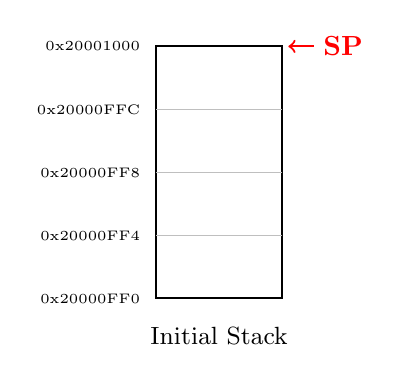
\begin{tikzpicture}[scale=0.8]
        % Stack frame
        \draw[thick] (0,0) rectangle (2,4);
        
        % Grid lines for 4 cells
        \foreach \y in {1,2,3} {
            \draw[thin, gray!50] (0,\y) -- (2,\y);
        }
        
        % Memory addresses (descending)
        \node[anchor=east] at (-0.1,4) {\tiny 0x20001000};
        \node[anchor=east] at (-0.1,3) {\tiny 0x20000FFC};
        \node[anchor=east] at (-0.1,2) {\tiny 0x20000FF8};
        \node[anchor=east] at (-0.1,1) {\tiny 0x20000FF4};
        \node[anchor=east] at (-0.1,0) {\tiny 0x20000FF0};
        
        % Stack pointer arrow
        \draw[->, thick, red] (2.5,4) -- (2.1,4);
        \node[right, red] at (2.5,4) {\textbf{SP}};
        
        % Title
        \node[below] at (1,-0.3) {\small Initial Stack};
    \end{tikzpicture}
    \caption{Initial empty stack}
    \label{fig:stack-initial}
\end{subfigure}
\hfill
\begin{subfigure}[t]{0.3\textwidth}
    \centering
    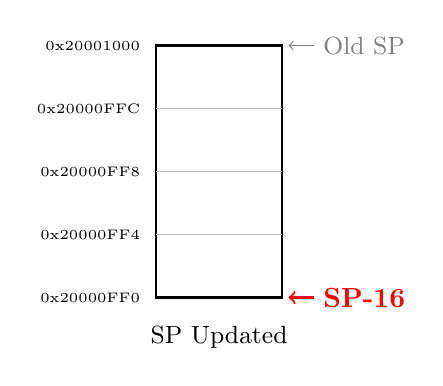
\begin{tikzpicture}[scale=0.8]
        % Stack frame
        \draw[thick] (0,0) rectangle (2,4);
        
        % Grid lines for 4 cells
        \foreach \y in {1,2,3} {
            \draw[thin, gray!50] (0,\y) -- (2,\y);
        }
        
        % Memory addresses (descending)
        \node[anchor=east] at (-0.1,4) {\tiny 0x20001000};
        \node[anchor=east] at (-0.1,3) {\tiny 0x20000FFC};
        \node[anchor=east] at (-0.1,2) {\tiny 0x20000FF8};
        \node[anchor=east] at (-0.1,1) {\tiny 0x20000FF4};
        \node[anchor=east] at (-0.1,0) {\tiny 0x20000FF0};
        
        % Old SP position (grayed out)
        \draw[->, thin, gray] (2.5,4) -- (2.1,4);
        \node[right, gray] at (2.5,4) {\small Old SP};
        
        % New SP position after PUSH {R0, R2, R4, LR}
        \draw[->, thick, red] (2.5,0) -- (2.1,0);
        \node[right, red] at (2.5,0) {\textbf{SP-16}};
        
        
        
        % Title
        \node[below] at (1,-0.3) {\small SP Updated};
    \end{tikzpicture}
    \caption{Stack pointer decremented}
    \label{fig:stack-sp-update}
\end{subfigure}
\hfill
\begin{subfigure}[t]{0.3\textwidth}
    \centering
    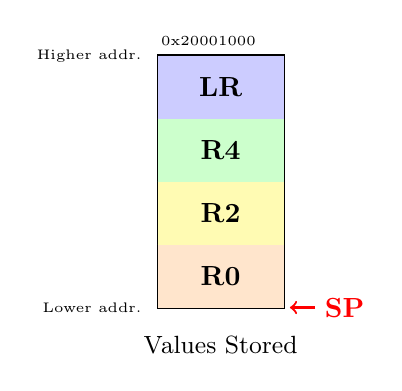
\begin{tikzpicture}[scale=0.8]
        % Stack frame
        \draw[thick] (0,0) rectangle (2,4);
        
        % Grid lines for 4 cells
        \foreach \y in {1,2,3} {
            \draw[thin, gray!50] (0,\y) -- (2,\y);
        }
        
        % Memory addresses (descending)
        \node[left, anchor=south west] at (-0.1,4) {\tiny 0x20001000};
        \node[left, anchor=south west] at (-0.1,3) {\tiny 0x20000FFC};
        \node[left, anchor=south west] at (-0.1,2) {\tiny 0x20000FF8};
        \node[left, anchor=south west] at (-0.1,1) {\tiny 0x20000FF4};
        \node[left, anchor=south west] at (-0.1,0) {\tiny 0x20000FF0};
        
        % Stored registers (in ascending order by number)
        \fill[blue!20] (0,3) rectangle (2,4);
        \node at (1,3.5) {\textbf{LR}};
        
        \fill[green!20] (0,2) rectangle (2,3);
        \node at (1,2.5) {\textbf{R4}};
        
        \fill[yellow!30] (0,1) rectangle (2,2);
        \node at (1,1.5) {\textbf{R2}};
        
        \fill[orange!20] (0,0) rectangle (2,1);
        \node at (1,0.5) {\textbf{R0}};
        
        % Stack pointer pointing to last used location
        \draw[->, thick, red] (2.5,0) -- (2.1,0);
        \node[right, red] at (2.5,0) {\textbf{SP}};
        
        % Annotations
        \node[left] at (-0.1,4) {\tiny Higher addr.};
        \node[left] at (-0.1,0) {\tiny Lower addr.};
        
        % Title
        \node[below] at (1,-0.3) {\small Values Stored};
    \end{tikzpicture}
    \caption{Registers stored in order}
    \label{fig:stack-values}
\end{subfigure}
\caption{Stack operation sequence for \texttt{PUSH \{R4, R0, R2, LR\}}}
\label{fig:stack-push-sequence}
\end{figure}

\noindent\textbf{Explanation:}
Figure~\ref{fig:stack-push-sequence}\textbf{(a)} shows the empty stack with \texttt{SP} at the top (highest address).
When \texttt{PUSH} executes, the processor \textbf{decrements \texttt{SP} by 16 bytes} to reserve space for four registers (Figure~\ref{fig:stack-push-sequence}\textbf{(b)}).
Finally, in Figure~\ref{fig:stack-push-sequence}\textbf{(c)}, values are stored according to the rule: the lowest-numbered register (R0) at the lowest address, then R2 and R4, and the highest-numbered (LR) at the highest address.
Because the stack grows downward, \texttt{SP} points to the last written word after the operation.

\bigskip
\paragraph{POP}

The \texttt{POP} instruction restores one or more registers from the stack.
Conceptually, the processor reads each value from the addresses currently covered by \texttt{SP} and then releases that stack space.
\textbf{Rule:} \texttt{POP} loads registers from the stack such that the \textbf{lowest-numbered register} is restored from the \textbf{lowest memory address}, and the \textbf{highest-numbered register} from the \textbf{highest memory address}.
After all specified registers are restored, \texttt{SP} has increased by 4 bytes per register.

\medskip
\noindent
\textbf{Example:}
\begin{lstlisting}
    POP {R6-R8}
\end{lstlisting}

This restores R6, then R7, then R8 from successively higher addresses; the stack pointer increases by 12 bytes overall.
If \texttt{PC} is included in the list, the loaded value becomes the new program counter, returning from the current procedure.

\begin{figure}[H]
\centering

\begin{subfigure}[t]{0.3\textwidth}
    \centering
    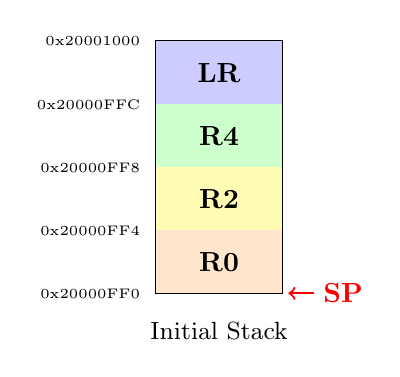
\begin{tikzpicture}[scale=0.8]
        % Stack frame
        \draw[thick] (0,0) rectangle (2,4);
        
        % Grid lines for 4 cells
        \foreach \y in {1,2,3} {
            \draw[thin, gray!50] (0,\y) -- (2,\y);
        }
        

        
        % Stored registers (in ascending order by number)
        \fill[blue!20] (0,3) rectangle (2,4);
        \node at (1,3.5) {\textbf{LR}};
        
        \fill[green!20] (0,2) rectangle (2,3);
        \node at (1,2.5) {\textbf{R4}};
        
        \fill[yellow!30] (0,1) rectangle (2,2);
        \node at (1,1.5) {\textbf{R2}};
        
        \fill[orange!20] (0,0) rectangle (2,1);
        \node at (1,0.5) {\textbf{R0}};
        
        % Stack pointer pointing to last used location
        \draw[->, thick, red] (2.5,0) -- (2.1,0);
        \node[right, red] at (2.5,0) {\textbf{SP}};
        
        % Annotations
        % Memory addresses (descending)
        \node[anchor=east] at (-0.1,4) {\tiny 0x20001000};
        \node[anchor=east] at (-0.1,3) {\tiny 0x20000FFC};
        \node[anchor=east] at (-0.1,2) {\tiny 0x20000FF8};
        \node[anchor=east] at (-0.1,1) {\tiny 0x20000FF4};
        \node[anchor=east] at (-0.1,0) {\tiny 0x20000FF0};
        
        % Title
        \node[below] at (1,-0.3) {\small Initial Stack};
    \end{tikzpicture}
    \caption{Initial stack after Figure \ref{fig:stack-push-sequence}}
\end{subfigure}
\hfill
\begin{subfigure}[t]{0.3\textwidth}
    \centering
    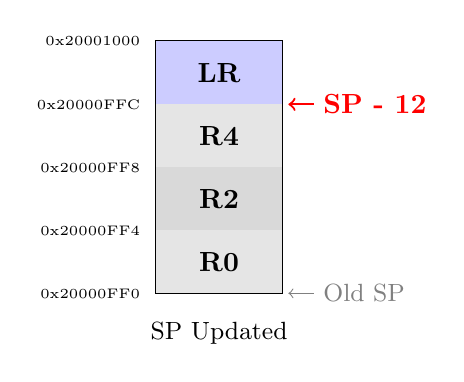
\begin{tikzpicture}[scale=0.8]
        % Stack frame
        \draw[thick] (0,0) rectangle (2,4);
        
        % Grid lines for 4 cells
        \foreach \y in {1,2,3} {
            \draw[thin, gray!50] (0,\y) -- (2,\y);
        }
        

        
        % Stored registers (in ascending order by number)
        \fill[blue!20] (0,3) rectangle (2,4);
        \node at (1,3.5) {\textbf{LR}};
        
        \fill[gray!20] (0,2) rectangle (2,3);
        \node at (1,2.5) {\textbf{R4}};
        
        \fill[gray!30] (0,1) rectangle (2,2);
        \node at (1,1.5) {\textbf{R2}};
        
        \fill[gray!20] (0,0) rectangle (2,1);
        \node at (1,0.5) {\textbf{R0}};
        
        % Stack pointer pointing to last used location
        \draw[->, thin, gray] (2.5,0) -- (2.1,0);
        \node[right, gray] at (2.5,0) {\small{Old SP}}; 

        \draw[->, thick, red] (2.5,3) -- (2.1,3);
        \node[right, red] at (2.5,3) {\textbf{SP - 12}};
        
        % Annotations
        % Memory addresses (descending)
        \node[anchor=east] at (-0.1,4) {\tiny 0x20001000};
        \node[anchor=east] at (-0.1,3) {\tiny 0x20000FFC};
        \node[anchor=east] at (-0.1,2) {\tiny 0x20000FF8};
        \node[anchor=east] at (-0.1,1) {\tiny 0x20000FF4};
        \node[anchor=east] at (-0.1,0) {\tiny 0x20000FF0};
        
        % Title
        \node[below] at (1,-0.3) {\small SP Updated};
    \end{tikzpicture}
    \caption{Stack pointer incremented}
\end{subfigure}
\hfill
\begin{subfigure}[t]{0.3\textwidth}
    \centering
    \centering
    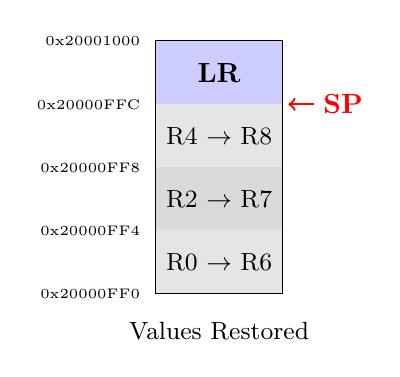
\begin{tikzpicture}[scale=0.8]
        % Stack frame
        \draw[thick] (0,0) rectangle (2,4);
        
        % Grid lines for 4 cells
        \foreach \y in {1,2,3} {
            \draw[thin, gray!50] (0,\y) -- (2,\y);
        }
        

        
        % Stored registers (in ascending order by number)
        \fill[blue!20] (0,3) rectangle (2,4);
        \node at (1,3.5) {\textbf{LR}};
        
        \fill[gray!20] (0,2) rectangle (2,3);
        \node at (1,2.5) {\small{R4 $\rightarrow$ R8}};
        
        \fill[gray!30] (0,1) rectangle (2,2);
        \node at (1,1.5) {\small{R2 $\rightarrow$ R7}};

        \fill[gray!20] (0,0) rectangle (2,1);
        \node at (1,0.5) {\small{R0 $\rightarrow$ R6}};
        
        % Stack pointer pointing to last used location
        \draw[->, thick, red] (2.5,3) -- (2.1,3);
        \node[right, red] at (2.5,3) {\textbf{SP}};
        
        % Annotations
        % Memory addresses (descending)
        \node[anchor=east] at (-0.1,4) {\tiny 0x20001000};
        \node[anchor=east] at (-0.1,3) {\tiny 0x20000FFC};
        \node[anchor=east] at (-0.1,2) {\tiny 0x20000FF8};
        \node[anchor=east] at (-0.1,1) {\tiny 0x20000FF4};
        \node[anchor=east] at (-0.1,0) {\tiny 0x20000FF0};
        
        % Title
        \node[below] at (1,-0.3) {\small Values Restored};
    \end{tikzpicture}
    \caption{Registers restored in order}
    \label{fig:stack-pop-restore}
\end{subfigure}

\caption{Stack operation sequence for \texttt{POP \{R6-R8\}}}
\label{fig:stack-pop-sequence}
\end{figure}
\noindent\textbf{Explanation:}
In Figure~\ref{fig:stack-pop-sequence}\textbf{(a)}, the stack contains values saved earlier.
Executing \texttt{POP \{R6-R8\}} \textbf{reclaims 12 bytes of stack space} (three registers) by moving \texttt{SP} upward in memory (Figure~\ref{fig:stack-pop-sequence}\textbf{(b)}).
Then, as shown in Figure~\ref{fig:stack-pop-sequence}\textbf{(c)}, registers are restored following the rule: the lowest-numbered register (R6) comes from the lowest address, followed by R7 and R8 from higher addresses.
After the last load, \texttt{SP} points to the top of the reclaimed block, completing the reversal of the earlier push.

\paragraph{Note:} This figure deliberately reuses the stack contents from the earlier \texttt{PUSH \{R0, R2, R4, LR\}} example, relabeling them R6/R7/R8 to illustrate that \texttt{POP} restores registers by \emph{address}, not by the name they were pushed under — it is not meant to represent the same code sequence continuing.



\newpage
\section{Procedure}

\subsection{Examples}

\subsubsection{Example 1: Nested Uppercase Counter}
This example demonstrates a nested call: \texttt{CountUpperNested(ptr)} scans a null-terminated string and calls \texttt{IsUpper(ch)} for each character. It shows saving/restoring \texttt{LR} and using callee-saved registers (\texttt{R4} for the running count, \texttt{R5} for the scan pointer). Both values must survive the \texttt{BL IsUpper} call, so under the AAPCS they cannot be kept in caller-saved registers like R0--R3. Compare it with Example 2 of Experiment 3, which counts the same letters inline with no procedures.
\lstinputlisting[caption={Nested procedure call to count uppercase letters}]{snippets/assembly/exp4/example1.asm}
\paragraph{Check:} Verify that \texttt{UPPERCOUNT} contains \texttt{5} for the test string.

\newpage
\subsubsection{Example 2: Integer to Decimal String with the Stack}
\texttt{UIntToStr(value, buf)} converts an unsigned integer into a null-terminated decimal ASCII string and returns the number of digits in R0. It finds each digit by dividing by 10 (\texttt{UDIV}, then \texttt{MLS} for the remainder), and this produces the digits in reverse order, least-significant first. Pushing each digit and then popping them all back reverses that order again, because the stack is last-in, first-out. Each \texttt{PUSH \{R12\}} takes a full 4-byte word even though it holds only one character. Because every push is matched by a pop, \texttt{SP} returns to its starting value before the final \texttt{POP \{R4, PC\}}.
\lstinputlisting[caption={Converting an integer to a decimal string using PUSH and POP}]{snippets/assembly/exp4/example2.asm}
\paragraph{Check:} Verify that R0 = 5 after the call, and open a Memory window at \texttt{NUMSTR} to confirm the bytes \texttt{34 30 32 31 33 00} (\texttt{"40213"}). Single-step the first loop with the Registers window open and watch \texttt{SP} drop by 4 for each digit. Then confirm that it climbs back during the second loop. Try the value 0 as well; the result should be \texttt{"0"}.

\newpage
\subsection{Tasks}

\subsubsection{Task 1: Count Vowels with Procedures}
Rewrite Task 1 of Experiment 3 as procedures:
\begin{itemize}[nosep]
    \item Create a procedure \texttt{IsVowel} that takes a character in R0 and returns 1 in R0 if it is a vowel (a, e, i, o, u, upper- or lowercase), and 0 otherwise.
    \item Create a procedure \texttt{CountVowels} that takes a string pointer in R0 and returns the number of vowels in R0, calling \texttt{IsVowel} for each character.
    \item Follow AAPCS conventions for parameter passing and register usage.
    \item Test it with the Experiment 3 string; the result must match your earlier answer.
\end{itemize}

\subsubsection{Task 2: Factorial Calculation (Recursive)}
\paragraph{Note on recursion:} Example 1's nested call has one procedure calling a \emph{different} one. In recursion, \texttt{FactorialRec} calls \emph{itself}. Each call needs its own copy of \texttt{LR} (and of any register it modifies) preserved across the inner call. So every invocation must \texttt{PUSH} its own \texttt{LR}, and usually the current \texttt{n} or partial result, before recursing, then \texttt{POP} them back on the way out. Because each active call keeps its own saved values on the stack, the recursion unwinds in reverse order as each \texttt{POP}/\texttt{BX LR} returns to its caller.

Implement a recursive procedure to calculate the factorial of a non-negative integer:
\begin{itemize}[nosep]
    \item Create a procedure \texttt{FactorialRec} that takes a non-negative integer in R0 and returns its factorial in R0.
    \item Use recursion to compute the factorial, with a base case that handles $0! = 1$.
    \item Manage the stack appropriately to save and restore registers as needed.
    \item Follow AAPCS conventions for parameter passing and register usage.
    \item Test the procedure with several inputs (including 0 and 1) to verify correctness.
\end{itemize}
